\documentclass[11pt]{article}
\usepackage{mypackages}
\begin{document}

% Max 

\section{Experiments and Expectations}

The aim of this project is to examine the effect of different amounts of threads
on the stability of deep reinforcement learning.
To acheive this we have solved both simple and advanced problems to investigate
the benefits and disadvantages of asynchronous training in two very different
settings.

\subsection{Solving CartPole using an Actor-Critic method with eligibility traces}

As a proof of concept we have implemented the method described in section
\ref{sec:actor_critic_el} for which the pseudo-code
can be found in appendix \ref{a:pseudo_code_et}.
The goal of this experiment is to show that a 
traditional Reinforcement Learning algorithm
is able to learn how to solve the CartPole problem, as well as provide a
baseline performance for the A3C algorithm.
I.e as a measure to test if A3C is performing at least as good
as the traditional/un-threaded Actor-Critic approach.

For this experiment we used two separate neural networks, with no
shared weights, as policy and state-value estimators.
The network that estimates the state-value function consisted of an
input layer with four entries, corresponding to the format of a state in CartPole,
followed by a single hidden layer with eight neurons, and an output layer of a single
neuron.
We used the RELU to activate the input to the
hidden layer and used a linear activation for the output neuron,
which means the neuron produced the weighted sum of its input as output.

For estimating the policy we used a network with the same structure,
with the only exception being that the output layer consists of two
neurons, each corresponding to the probability of picking an action.
To emulate the probability distribution we used the softmax function
to activate the final layer.

When we implemented the algorithm, we ran into some trouble with
the state-value estimator sometimes becoming too large, resulting
in both the probabilties and state-value estimates throwing a \texttt{NaN} error,
meaning they couldn't be represented using the bits they were assigned.
Therefore we had to restrict the parameters of the algorithm to
be small, which might cause the results of the
experiment being at a disadvantage, compared to our A3C implementation, since the learning happend
at a slower pace than could be achieved with a better implementation.

\subsection{Solving CartPole using the A3C algorithm}

To examine the effect of asynchronous training in a simpler setting than
the Atari games, we have implemented the A3C algorithm presented
in \cite{a3c} and given by the pseudo-code from appendix \ref{a:pseudo_code_a3c}.

We have chosen to also solve the CartPole problem with this approach, as a way to
investigate how asynchronous training influences the stability of the algorithm,
compared to the more traditional Actor-Critic approach, and 
to itself with different amounts of threads.

As in the previous implementation we ecnountered the \texttt{NaN} error,
but to a much lesser degree.
This means that the error should have little to no impact on
the final results.

To estimate the policy and state-value functions we used a single
neural network.
The structure of the network resembles the structure used in the traditional
Actor-Critic method, with the key difference being that the network has
two output layers

\begin{figure}[H]
    \centering
    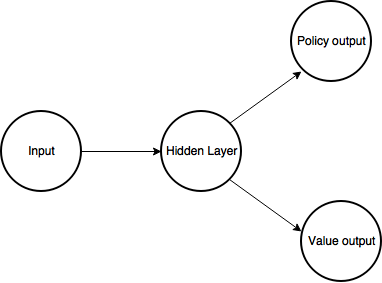
\includegraphics[scale=0.5]{include/shared_cartpole.png}
    \caption{The neural network used to estimate both the state-value
             and policy functions.}
    \label{fig:s_cartpole}
\end{figure}

For both the CartPole problem and the Atari games we will be using the same asynchronous setup
as described in \cite{a3c}.
This means that we will be using a single global network, whose only
purpose is to keep track of a set of global weights, and a local network
for each thread.
To perform the asynchronous update of the global weights we will be using
RMSpropagation as described in section \ref{sec:a3c}.
The parameters of the RMSpropagation, and the algorithm in general, have
been chosen because they provide decent test results.
Due to the time limitations of the project we haven't performed
a more sophisticated selection of the parameters, which might
influence the results of the experiments.

\subsection{Solving Atari Games}

To make sure the advantages and disadvantages of asynchronous training
is thouroughly inverstigated we have also implemented the A3C algorithm
to learn in the more advanced setting of Atari games.

We will be examining the effect of different amounts of threads
in Space Invader and Breakout.
The main difference between this implementation of A3C
and the one we used to play CartPole is the structure of the
policy and value estimators.
Again we have used a single network with two output layers,
but for this setting we have used the setup presented
in detail in \cite{dqn-nature}.
Thus the network consists of an input layer, that takes a $84 \times 84 \times 4$
image-stack as input.
Instead of feeding the network a single frame from an Atari game,
we stack the four latest frames in an attempt to let the network
experience the movement of objects in the frame.
This layers is followed by a convolutional layer that reduces the dimensions
of the input in both directions by a factor of four.
The layer produces 16 $21 \times 21$ feature maps using 16 kernel filters,
which is then set to another convolutional layer..
This layer halves the size of the image, and produces 32 $11 \times 11$
feature maps.
Both of the convolutional layers activated their input using the
RELU function.
After the second convolution, we flatten the output resulting in
$11 * 11 * 32 = 3872$ neurons, which are fully connected to
a layer with 256 neurons.
In this layer the input is again activated using the RELU and
the output is then sent to two different layers.
One of the layers consists of only a single neuron
and simply outputs the weighted sum of its input as the estimated value
of the image-stack the network was originally presented.
The other output layer activates its input using the softmax function,
using as many neurons as there are actions available, with the output of
each neuron representing the probability of taking an action.
A representation of the network is shown below.

\begin{figure}[H]
    \centering
    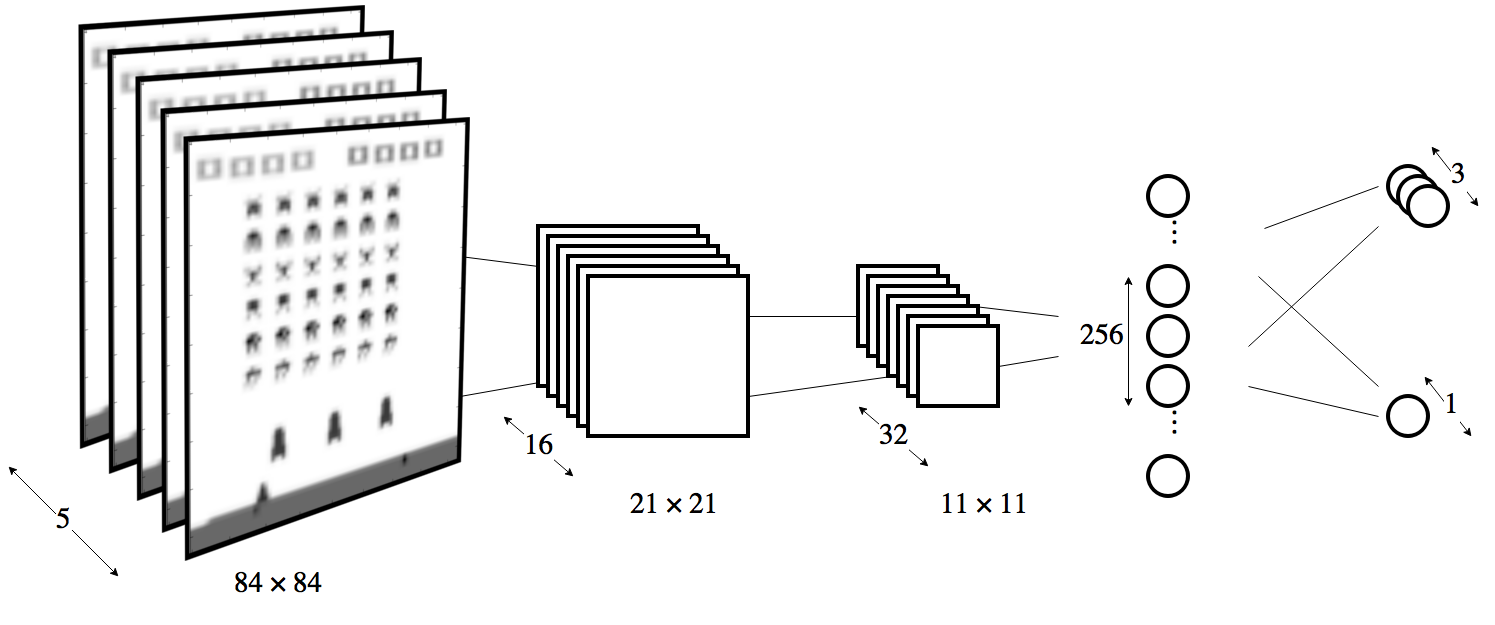
\includegraphics[scale=0.25]{include/Atari_network.png}
    \caption{The neural network used to estimate both the state-value
             and policy functions for Atari games. In this example the network
             is used on Space Invaders which means it has to assign each of three actions a probability.}
    \label{fig:atari_network}
\end{figure}

Taking an action using the OpenAI framework only leads to a small change in states,
since it is only performed for two to four frames.
To increase the impact of taking an action we have used the same \textit{action repeat}
stategy as described in \cite{a3c}, which means that an action is performed four times
after being sampled.
Even though openAI returns a new state every time the action is taken, we only consider
the fourth state as the one the action lead to, but we accumulate the rewards that
we are given during the action repeat, since they are a product of the action.

In Space Invaders we perform two additional preprocessing steps before
the network is fed any state.
The rewards that can be obtained vary based on what the learning agent “hits”
in the environment.
The optimal strategy is however to shoot all aliens in a level, and not focus on
hitting only the ones that produce the greatest reward.
Therefore we have chosen to clip the rewards returned by the environment, such that
the rewards always lie between $-1$ and $1$.

A problem with Space Invaders is that the screen sometimes flicker.
Thus some of the frames might not contain a “player”.
To avoid this issue we always define a state as the pixel-wise maximum
between the previous frame and the current frame.

\end{document}
